\begin{frame}
\setbeamercovered{invisible}
\begin{adjustwidth}{-2.5em}{-2.5em}

% Set the overall layout of the tree
% \tikzstyle{level 1}=[level distance=7em, sibling distance=11em]
% \tikzstyle{level 2}=[level distance=9em, sibling distance=4em]
\tikzstyle{level 1}=[level distance=8em, sibling distance=12em]
\tikzstyle{level 2}=[level distance=11em, sibling distance=5em]

% Define styles
\tikzstyle{root} = []
\tikzstyle{internal} = []
\tikzstyle{tip} = [text width = 3.5em]
\tikzstyle{branch} = [->, very thick]

\uncover<6->{
% \begin{center}
\hspace{0.5\textwidth}
    {\LARGE $\boldsymbol{\alpha =} \only<6>{\mathbf{\conc}}\only<7->{\mathbf{\cconc}}$} \\
% \end{center}
}

\noindent
\begin{tikzpicture}[grow=right]%, sloped]
\pgfkeys{/pgf/number format/.cd,fixed,fixed zerofill,precision=3}
% \pgfkeys{/pgf/number format/.cd,std,fixed zerofill,precision=3}
\node[root] {\lclass{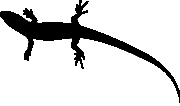
\includegraphics[angle=-90,origin=c,height=6mm]{../images/lizard-1.pdf}}{}{}}
    child [visible on=<2->]{
        node[internal] {\lclass{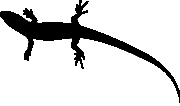
\includegraphics[angle=-90,origin=c,height=6mm]{../images/lizard-1.pdf}}{
\includegraphics[angle=90,origin=c,height=6mm]{../images/lizard-2.pdf}}{}}
            child [visible on=<4->]{
                node[tip, label=right:
                    {\tiplabel{\uncover<5->{
                        $
                        % p(m = 123)=
                        \left(\frac{\alpha}{\alpha+1}\right)\left(\frac{\alpha}{\alpha+2}\right)
                        \only<6>{= \calcprob{\conc}{\conc}}
                        \uncover<7->{= \ccalcprob{\cconc}{\cconc}}$
                        }}}]
                    {\lclass{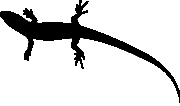
\includegraphics[width=6mm]{../images/lizard-1.pdf}}{
\includegraphics[width=6mm]{../images/lizard-2.pdf}}{
\includegraphics[width=6mm]{../images/lizard-3.pdf}}}
                edge from parent [style = branch]
                node[above,
                    label={[label distance = -0.5em]\branchlabel{$\frac{\alpha}{\alpha+2}$}}
                    ] {}
            }
            child [visible on=<4->]{
                node[tip, label=right:
                    {\tiplabel{\uncover<5->{
                        $
                        % p(m = 121)=
                        \left(\frac{\alpha}{\alpha+1}\right)\left(\frac{1}{\alpha+2}\right)
                        \only<6>{= \calcprob{\conc}{1}}
                        \uncover<7->{= \ccalcprob{\cconc}{1}}$
                        }}}]
                    {\pclass{AC}{B}{}}
                edge from parent [style = branch]
                node[above,
                    label={[label distance = -0.5em]\branchlabel{$\frac{1}{\alpha+2}$}}
                    ] {}
            }
            child [visible on=<4->]{
                node[tip, label=right:
                    {\tiplabel{\uncover<5->{
                        $
                        % p(m = 122)=
                        \left(\frac{\alpha}{\alpha+1}\right)\left(\frac{1}{\alpha+2}\right)
                        \only<6>{= \calcprob{\conc}{1}}
                        \uncover<7->{= \ccalcprob{\cconc}{1}}$
                        }}}]
                     {\pclass{A}{BC}{}}
                edge from parent [style = branch]
                node[above,
                    label={[label distance = 0em]\branchlabel{$\frac{1}{\alpha+2}$}}
                    ] {}
            }
            edge from parent [style = branch]
            node[above,
                label={[label distance = 0em]\branchlabel{$\frac{\alpha}{\alpha+1}$}}
                ] {}
    }
    child [visible on=<2->]{
        node[internal] {\pclass{AB}{}{}}        
            child [visible on=<3->]{
                node[tip, label=right:
                    {\tiplabel{\uncover<5->{
                        $
                        % p(m = 112)=
                        \left(\frac{1}{\alpha+1}\right)\left(\frac{\alpha}{\alpha+2}\right)
                        \only<6>{= \calcprob{1}{\conc}}
                        \uncover<7->{= \ccalcprob{1}{\cconc}}$
                        }}}]
                    {\pclass{AB}{C}{}}
                edge from parent [style = branch]
                node[above,
                    label={[label distance = -0.5em]\branchlabel{$\frac{\alpha}{\alpha+2}$}}
                    ] {}
            }
            child [visible on=<3->]{
                node[tip, label=right:
                    {\tiplabel{\uncover<5->{
                        $
                        % p(m = 111)=
                        \left(\frac{1}{\alpha+1}\right)\left(\frac{2}{\alpha+2}\right)
                        \only<6>{= \calcprob{1}{2}}
                        \uncover<7->{= \ccalcprob{1}{2}}$
                        }}}]
                    {\pclass{ABC}{}{}}
                edge from parent [style = branch]
                node[above,
                    label={[label distance = -0.5em]\branchlabel{$\frac{2}{\alpha+2}$}}
                    ] {}
            }
            edge from parent [style = branch]
            node[above,
                label={[label distance = 0em]\branchlabel{$\frac{1}{\alpha+1}$}}
                ] {}
    };
\end{tikzpicture}

\end{adjustwidth}
\end{frame}

